\chapter{Language Implementation}


\section{Data Type}
\subsection{Tokenizer Type}
All tokens are define using the Haskell Lexer Generator Alex.Tokens will be recognized and converted to Haskell data types.For example , a valid variable is comprised with one or more alphabetic characters and digit and the first character must be an alphabetic characters. This rule can be defined as ,
\begin{lstlisting}[language=java]
$digit = 0-9			-- digits
$lowerCase = [a-z]
$alpha = [a-zA-Z]		-- alphabetic characters

tokens :-
  $alpha [$alpha $digit \_ \' \.]* { \s -> TName s }
-- data definition
data Token = 
	TName String |
	TBool Bool  | 
	TInt Int  | 
	...  -- more definition			

\end{lstlisting}

The variable \textbf{var1} will be parse into Haskell data type \textbf{TName "var1"}\\


By using the lexer , all the code will be generated into tokens streams.
\begin{lstlisting}[language=java]
program myProgram ()
{
	var1 = 1;
	result = var1 + "a string";
}
\end{lstlisting}

The following codes show the invocation of the lexer and the returned tokens stream.
\begin{lstlisting}[language=java]
lexer "program myProgram() { var1 = 1; result = var1 + False; return 0; }"
[TProgram,TName "myProgram",TOPB,TCPB,TOCB,TName "var1",TAssign,TInt 1,TSC,TName "result",TAssign,TName "var1",TPlus,TBool False,TSC,TReturn,TInt 0,TSC,TCCB]
\end{lstlisting}



\subsection{Parser internal data type}
The Parser internal data type typically represents a parse tree.To represent a generic expression,we can define data type as follow,

\begin{hcode}
data GenericExp  =
		     Var String 
		   | Int Int
		   | Double Double
		   | Plus GenericExp GenericExp		   
		   | ListIndex String [GenericExp]
		   | Brack GenericExp  deriving 
		   ... -- more definition
\end{hcode}


The following code 
\begin{lstlisting}[language=java]
( a +1 )  /=  3
myArray[ 1+1,2] 
\end{lstlisting}

are parsed into Haskell data structure,

\begin{hcode}
NotEq  (Brack ( Plus (Var "a") (Int 1)))  (Int 3)
ListIndex "myIndex" [ Plus (Int 1) (Int 1) , Int 2 ] 
\end{hcode}


\begin{figure}[H]
  \centering
	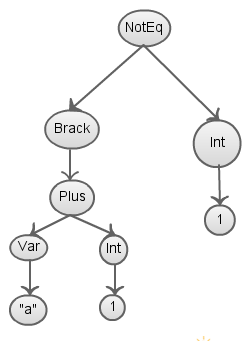
\includegraphics[width=0.40\textwidth]{pic/c6/parse_tree_1.png}
	\caption{Diagram illustrating a parse tree of a generic expression}
\end{figure}


In Haskell,a parse tree data structure that support polymorphic list can be defined using recursive data type as follow, 
\begin{hcode}
data List = ListGenericExp GenericExp
			| ListList [List] deriving (Show,Eq,Read)  
\end{hcode}


A polymorphic list,
\begin{lstlisting}[language=java]
 [1,2,["string",2,3]];
\end{lstlisting}

Can be represent in Haskell data type.

\begin{hcode}
ListList  [ListGenericExp (Int 1),ListGenericExp (Int 2),
	ListList [ListGenericExp String "string",
		ListGenericExp (Int 2),ListGenericExp (Int 3)]] 
\end{hcode}



\begin{figure}[H]
  \centering
	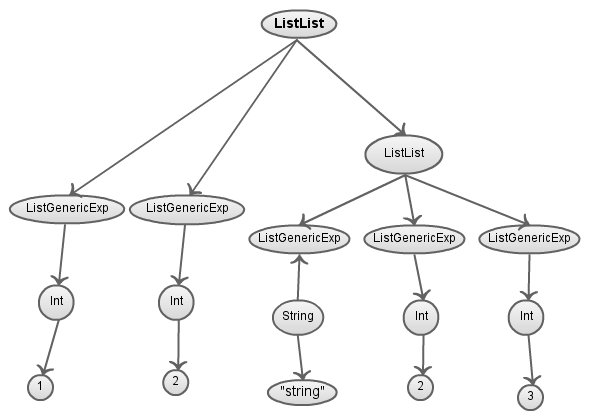
\includegraphics[width=0.90\textwidth]{pic/c6/parse_tree_2.png}
	\caption{Diagram illustrating a parse tree of a list expression}
\end{figure}


\subsection{Interpreter Internal Data Type}
The data type defined as below shows that the possible data type of result that a sub-interpreter will return.There is a interpreter correspond it.The sub-interpreter will return for example an interger to represent the result of a generic expression.The recursive data type is use for a the purpose of nested list support. 
\begin{hcode}
data Value =  Int Int 
             | Bool Bool
             | Double Double
             | String String 
             | List [Value]
             | NULL    deriving Show
\end{hcode}


\subsubsection{The Interpreter Monad}
The interpreter monad is a combination of Error Monad ,State Monad and IO monad.

\begin{hcode}
type Interp a  = (ErrorT String (StateT Storage IO )) a

type SymbolTable = M.Map String Value
type Storage = (SymbolTable,[Func])
\end{hcode}


For each sub-interpreter ,it must accept an expression and return a \textbf{Interp} type.The \textbf{Interp} type is a monad constructor that offer encapsulation support to return value.One of the \textbf{StateT} parameter is the type \textbf{Storage} which represents the internal storage of an interpreter like symbol table and parse tree of sub-function.



\section{Module Evaluator}
Module is the minimum executable unit in \textbf{yun} programming language.A module is comprised by one main function and multiple sub functions.What the Module Evaluator will do is ,first initial the symbol table using a empty map, second, extract the parse tree data and put in two together with the symbol table,third,extract all statements in main function and hand it over to statement evaluator.This Evaluator will not check the error message from other sub-evaluator it invoked,all the error will be passed to the main function.
\begin{figure}[H]
  \centering
	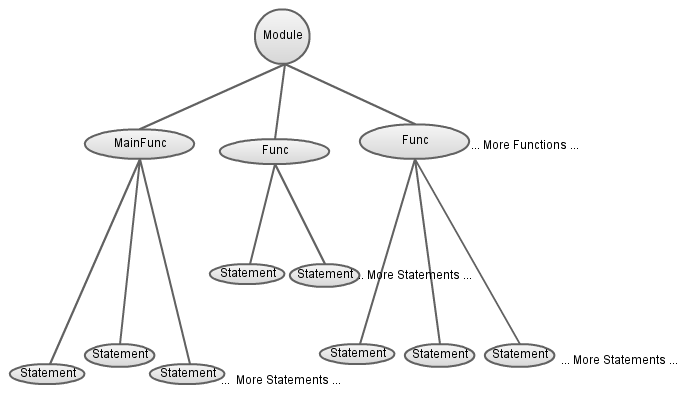
\includegraphics[width=0.90\textwidth]{pic/c6/module.png}
	\caption{Diagram illustrating a parse tree of a module}
\end{figure}
\section{Statement Evaluator}


\begin{hcode}
data Control = Break | Continue | DoNothing | Return Value deriving (Show)

stmtsEval :: [Stmt] -> Interp Control
stmtsEval --   function body

stmtEval :: Stmt -> Interp Control
stmtEval  -- the function body
\end{hcode}
\textbf{Stmt} is a data type that represents a Parse Tree of a statement.The first statement evaluator will accept a list of statement and for each statement,it invoke the statement evaluator.By applying patter matching,the statement will do correspond action toward each type of the statement.For example, for the \textbf{break} or \textbf{continue} statements,it will return the corresponding control command.The diagram below illustrate the how the statement evaluator works.

\begin{figure}[H]
  \centering
	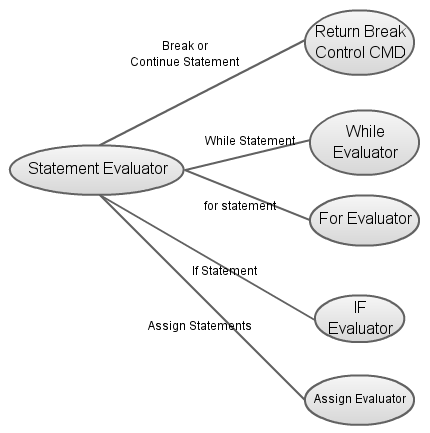
\includegraphics[width=0.80\textwidth]{pic/c6/statement.png}
	\caption{Diagram illustrating guard condition and function invocation}
\end{figure}




\section{Symbol Table and Parse Tree}
The symbol table together with the parse trees of sub-functions as a tuple will be stored behind the state monad.Symbol table is a map that mapping from a string to the type \textbf{Value} mentioned above.Monadic function composed to support add ,update from the symbol table.

\begin{hcode}
type SymbolTable = M.Map String Value
type Storage = (SymbolTable,[Func])
type Interp a  = (ErrorT String (StateT Storage IO )) a
\end{hcode}


\section{Generic Expression Evaluator}
The generic evaluator supports evaluation of internal data type like string ,integer ,double and list.As \textbf{yun} is a weak typing language ,the generic expression will do the internal type conversions. For example,a expression like \textbf{"string" + 1 } will be evaluator to  \textbf{"string1"}.All value can be converted to a string generally,but not all the value can be convert to an integer.The follow expression \textbf{1+True} will cause an error.

Importantly,as weak typing languages have their own conversion rule,type conversion is somewhat unpredictable thus relying on type conversion is not recommended.


\section{Function Invocation}
Different from most of imperative language, \textbf{yun} only supports pass by value parameter passing.To invoke a function,it is  needed to save the current scene and initialize the variable table for the function.



\section{Main Function}
The main function will load the source code, the it will invoke the parser which turns source code into a parse tree.Afterwards,the module evaluator will be invoke.


